\documentclass[11pt,presentation]{beamer}   % to compile the presentation
% \documentclass[handout]{beamer}        % to compile 2x2 handouts
\usepackage[ansinew]{inputenc}
\usepackage[T1]{fontenc}
\usepackage{lmodern,textcomp}
\usepackage{breakurl}
\usepackage{listings}                 	% Source code printer for LaTeX
\usepackage{xcolor}                   	% Support for using colours
\usepackage[noabbrev,nameinlink]{cleveref}   % Clever references. Options: "fig. [1]" --> "[Figure 1]"
\usepackage{wrapfig}
\usepackage{graphicx}
\usepackage{float}
\usepackage{xcolor}

\usepackage{tikz}
\usetikzlibrary{arrows,shapes,positioning,topaths}

\definecolor{dtured}{cmyk}{0,.91,.72,.23}
\definecolor{dtugray}{cmyk}{0,0,0,.56}
\definecolor{s05}{cmyk}{.0,1,.0,.0}    % magenta
\definecolor{s06}{cmyk}{.25,1,.0,.0}
\definecolor{s07}{cmyk}{.25,1,0,0}
\definecolor{s08}{cmyk}{.75,1,0,0}
\definecolor{s09}{cmyk}{.75,.75,.0,.0}
\definecolor{s10}{cmyk}{.5,0,0,0}
\definecolor{s11}{cmyk}{.5,.0,.0,.0}
\definecolor{s13}{cmyk}{.75,.50,.0,.0} % blue
\definecolor{s14}{cmyk}{.5,0,1,0}      % green
\definecolor{s14a}{cmyk}{.6,0,1,.25}      % green


%%%%%%%%%%%%
% Listings %
%%%%%%%%%%%%
\crefname{lstlisting}{listing}{listings}
\Crefname{lstlisting}{Listing}{Listings}

\usetheme{dtu}

\graphicspath{{img/}}

\newcommand{\comm}[1]{}
\AtBeginSection[]
{
 \begin{frame}<beamer>
 \frametitle{Outline}
 \tableofcontents[currentsection]
 \end{frame}
}

\newcommand {\framedgraphic}[2] {%
    \begin{frame}{#1}%
        \begin{center}%
            \includegraphics[width=1.0\textwidth,height=0.75\textheight,keepaspectratio]{#2}%
        \end{center}
    \end{frame}
}
%\framedgraphic{OCL: Enterprise Report}{Class_Diagram/OCLEnterpriseReport}


\begin{document}

% The DTU and MIC logos
\pgfdeclareimage[height=2.0cm]{dtulogo}{dtu_logo}

% % % % % % % % % % % % % % % % % % % % % % % % % % % % % % % % % % % % % % % % % % % % % % % % % %


\begin{frame}{Find all spanning trees}

\begin{figure}[H]
\centering
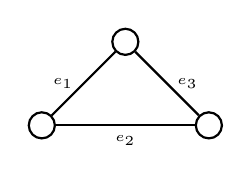
\begin{tikzpicture}[auto,node distance=1.5cm,
  thick,main node/.style={circle,draw,font=\sffamily\tiny\bfseries}]
  \node[main node] (1) {};
  \node[main node] (2) [above right of=1] {};
  \node[main node] (3) [below right of=2] {};
% \node[main node] (4) [right of=3] {4};

  \path[every node/.style={font=\sffamily\tiny}]
  (1) edge node [left] {$e_1$} (2)
    	edge [right] node [below] {$e_2$} (3)
    (2) edge node [right] {$e_3$} (3);
    %	edge [bend left] node {0} (4)
   % (3) edge node {$s_2$} (4);

\end{tikzpicture}
\label{fig:example}
\end{figure}

\hrule

\begin{figure}[H]
\resizebox{\linewidth}{!}{
\centering
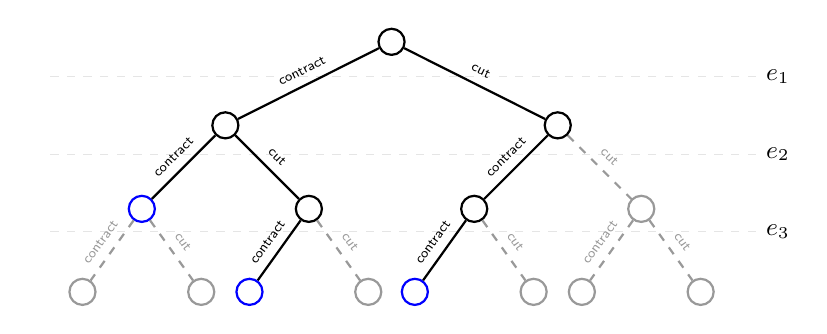
\begin{tikzpicture}[auto,node distance=1.5cm,font=\sffamily\tiny,
  thick,main node/.style={circle,draw,font=\sffamily\tiny},
  edge label/.style={midway,above,sloped,font=\sffamily\tiny}]

  \node[main node] (1) {};
  \node[node distance=1.05cm] (1a) [left of=1] {};
  \node[node distance=1.05cm] (1b) [right of=1] {};
  \node[main node] (2) [below left of=1a] {};
  \node[main node] (3) [below right of=1b] {};
  
  \node[main node,blue] (4) [below left of=2] {};
  \node[main node] (5) [below right of=2] {};
  \node[main node] (6) [below left of=3] {};
  \node[main node,opacity=0.4] (7) [below right of=3] {};
  
  \node[main node,opacity=0.4] (8) [below left=0.8cm and 0.5cm of 4] {};
  \node[main node,opacity=0.4] (9) [below right=0.8cm and 0.5cm of 4] {};
  \node[main node,blue] (10) [below left=0.8cm and 0.5cm of 5] {};
  \node[main node,opacity=0.4] (11) [below right=0.8cm and 0.5cm of 5] {};
  \node[main node,blue] (12) [below left=0.8cm and 0.5cm of 6] {};
  \node[main node,opacity=0.4] (13) [below right=0.8cm and 0.5cm of 6] {};
  \node[main node,opacity=0.4] (14) [below left=0.8cm and 0.5cm of 7] {};
  \node[main node,opacity=0.4] (15) [below right=0.8cm and 0.5cm of 7] {};
  
  \draw (1) -- (2) node[edge label] {contract};
  \draw (1) -- (3) node[edge label] {cut};
  
  \draw (2) -- (4) node[edge label] {contract};
  \draw (2) -- (5) node[edge label] {cut};
  \draw (3) -- (6) node[edge label] {contract};
  \draw[dashed,opacity=0.4] (3) -- (7) node[edge label] {cut};
  
  \draw[dashed,opacity=0.4] (4) -- (8) node[edge label]{contract};
  \draw[dashed,opacity=0.4] (4) -- (9) node[edge label] {cut};
  \draw (5) -- (10) node[edge label] {contract};
  \draw[dashed,opacity=0.4] (5) -- (11) node[edge label] {cut};
  \draw (6) -- (12) node[edge label] {contract};
  \draw[dashed,opacity=0.4] (6) -- (13) node[edge label] {cut};
  \draw[dashed,opacity=0.4] (7) -- (14) node[edge label] {contract};
  \draw[dashed,opacity=0.4] (7) -- (15) node[edge label] {cut};
 
 
  \node[font=\small] (L1) [below right=0.1cm and 4.5cm of 1] {$e_1$};
  \node[font=\small] (L2) [below=0.55cm of L1] {$e_2$};
  \node[font=\small] (L3) [below=0.55cm of L2] {$e_3$};

  \node[] (La1) [left=9cm of L1] {};
  \node[] (La2) [left=9cm of L2] {};
  \node[] (La3) [left=9cm of L3] {};
  
  \draw[dashed, thin, opacity=0.1] (L1) -- (La1);
  \draw[dashed, thin, opacity=0.1] (L2) -- (La2);
  \draw[dashed, thin, opacity=0.1] (L3) -- (La3);
\end{tikzpicture}}
\label{fig:comptree}
\end{figure}

\end{frame}

\begin{frame}{Techniques/tricks used}
\begin{itemize}[<+->]
\item \textbf{Heuristic:} $\max\{w(e_i), w(e_{m-i-1})\}$
\item \textbf{Checking cut:} DFS, matrix to end search for other node faster
\item \textbf{Checking cycles:} Persistent Union-Find data structure
\item Pruning of computation tree using current best B
\item Arrays used as main data structures: fast look-up and modification
\item Fixed memory usage based on edges and nodes -- all allocated at initialization
\end{itemize}
\end{frame}


\end{document} 
